\graphicspath{{Figures/}}

\title{\fontsize{33}{45}{\huge Getting Started in Python\newline \vspace{8pt} \Large  using Anaconda \vspace{-1.1cm}
}}

\vspace{0.5cm}
\author{\vspace{0.4cm}\\\large{\bf Kundan Kumar\\\url{https://github.com/erkundanec/PatternClassification}}
%Associate Professor\\Department of ECE}
}
% - Give the names in the same order as the appear in the paper.
% - Use the \inst{?} command only if the authors have different
%   affiliation.
%\vspace{1cm}
\institute[Indian Institute of Technology Kharagpur] % (optional, but mostly needed)
{
\vspace{1.8cm}
%\includegraphics[height=.17\textheight]{SOAlogo.png}\\
% Faculty of Engineering (ITER)\\ S`O'A Deemed to be University, Bhubaneswar, India-751030\\


 \copyright\  2020 Kundan Kumar, All Rights Reserved\\
  \vspace{-1.1cm}}
% - Use the \inst command only if there are several affiliations.
% - Keep it simple, no one is interested in your street address.
\date{}
% To remove page number from a perticular slide
{
\setbeamertemplate{logo}{}
\makeatletter
\setbeamertemplate{footline}{
        \leavevmode%
  
  % First line.
  \hbox{%
  \begin{beamercolorbox}[wd=.2\paperwidth,ht=\beamer@decolines@lineup,dp=0pt]{}%
  \end{beamercolorbox}%
  \begin{beamercolorbox}[wd=.8\paperwidth,ht=\beamer@decolines@lineup,dp=0pt]{lineup}%
  \end{beamercolorbox}%
  } %
  % Second line.
  \hbox{%
  \begin{beamercolorbox}[wd=\paperwidth,ht=\beamer@decolines@linemid,dp=0pt]{linemid}%
  \end{beamercolorbox}%
  } %
  % Third line.
  \hbox{%
  \begin{beamercolorbox}[wd=.1\paperwidth,ht=\beamer@decolines@linebottom,dp=0pt]{}%
  \end{beamercolorbox}%
  \begin{beamercolorbox}[wd=.9\paperwidth,ht=\beamer@decolines@linebottom,dp=0pt]{linebottom}%
  \end{beamercolorbox}%
  }%
        }
\makeatother
\begin{frame}
\titlepage
\end{frame}
}
\section{Introduction}
\subsection{}
\begin{frame}{Introduction}
\begin{itemize}
\item Anaconda is an open-source distribution for python and R.
\begin{figure}

\includegraphics[scale=0.5]{Anaconda.png}
\end{figure}
\item It is used for 
\begin{itemize}
\item data science, 
\item machine learning, 
\item deep learning, etc. 
\end{itemize}
\item More than 300 libraries are available for data science.
\item Simplified package management and deployment.
\item An easily manageable environment setup which can deploy any project with the click of a single button.
\end{itemize}
\end{frame}

\section{Installation And Setup}
\subsection{}

\begin{frame}{Where to find Anaconda?}
\begin{itemize}
\item[1.] Go to website: {\color{blue}\url{https://www.anaconda.org}}
\item[2.] Click on download on top-right corner and scroll down.
\begin{figure}
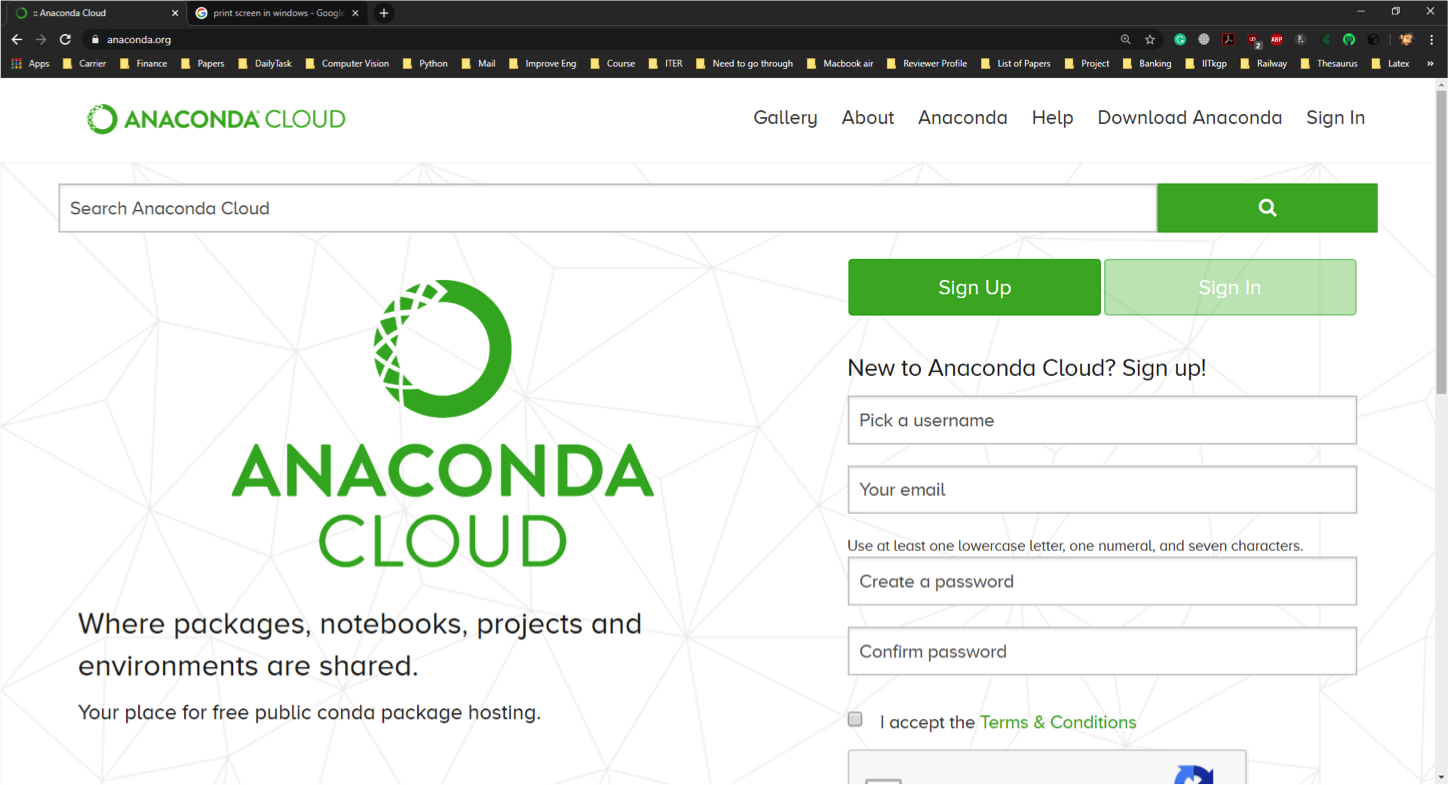
\includegraphics[width=\textwidth]{python001.png}
\end{figure}
\end{itemize}
\begin{tikzpicture}[remember picture, overlay]
%\draw[help lines,black] (0,0) grid (11,7);
\draw[draw=red,rounded corners=2pt,line width=1pt]  (1,6.2) rectangle ++(3,0.3);

\node[circle,draw=white, line width=1pt, inner sep=1pt,minimum size=12pt] (1) at(4.4,6.4) {\color{white}1};

\node[circle,draw=black, line width=1pt, inner sep=1pt,minimum size=12pt] (1) at(10.9,5.5) {\color{black}2};

\draw[draw=red,rounded corners=2pt,line width=1pt] (8.85,5.6) rectangle ++(1.7,0.3);
\end{tikzpicture}
\end{frame}



\begin{frame}{Where to find Anaconda?}
\begin{itemize}
\item[3.] Choose your operating system.
\item[4.] Download 64-Bit or 32-Bit Graphical Installer (Python 3.7 version).
\begin{figure}
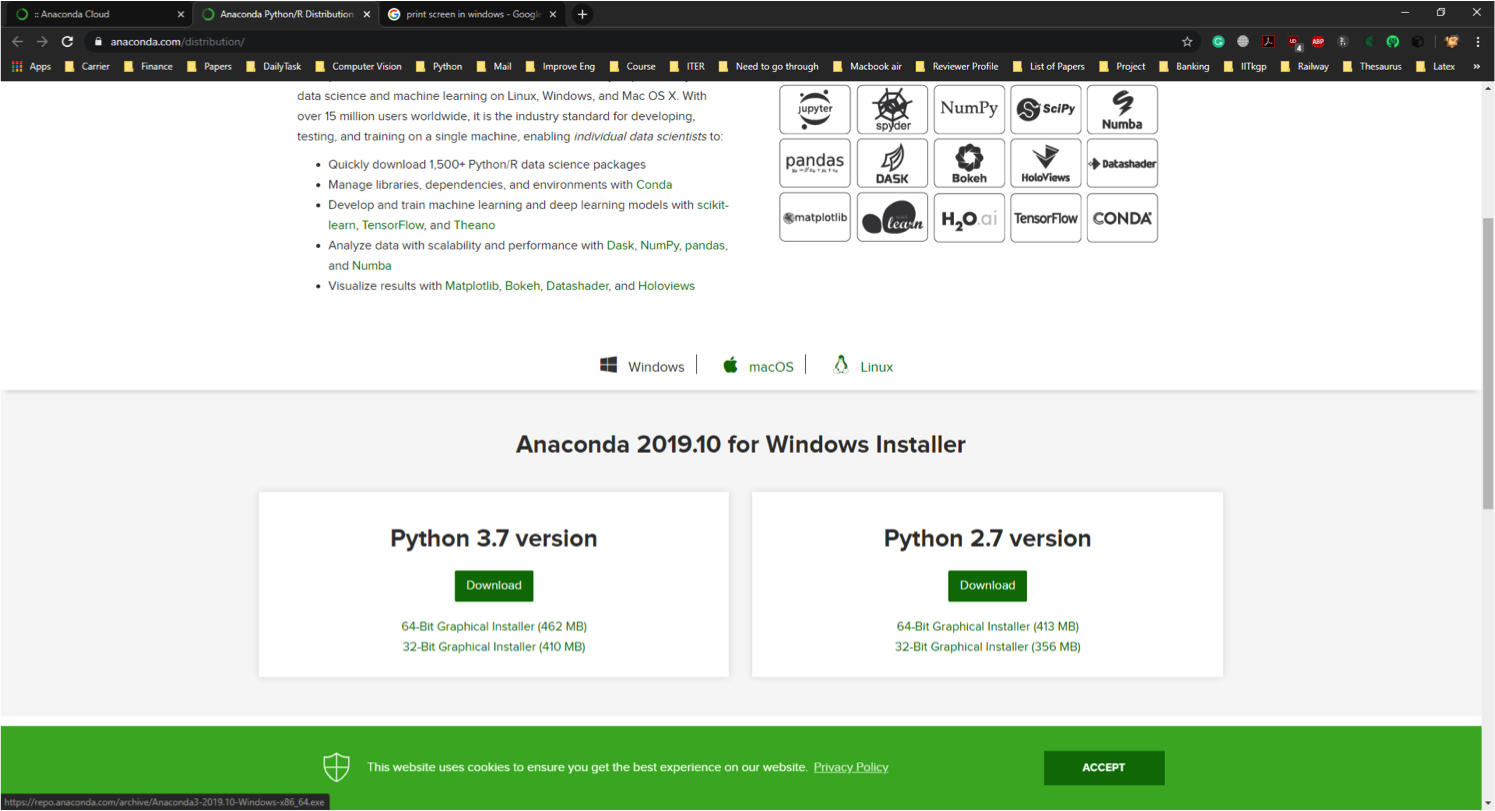
\includegraphics[width=\textwidth]{python002.png}
\end{figure}
\end{itemize}
\begin{tikzpicture}[remember picture, overlay]
%\draw[help lines,black] (0,0) grid (11,7);
\draw[draw=red,rounded corners=2pt,line width=1pt]  (3.5,2.1) rectangle ++(1.5,0.3);

\node[circle,draw=black, line width=1pt, inner sep=1pt,minimum size=12pt] (1) at(5.45,2.15) {\color{black}4};

\draw[draw=red,rounded corners=2pt,line width=1pt]  (4.9,3.75) rectangle ++(2.5,0.3);

\node[circle,draw=black, line width=1pt, inner sep=1pt,minimum size=12pt] (1) at(7.9,4) {\color{black}3};
\end{tikzpicture}
\end{frame}


\section{Install Anaconda}
\subsection{}
\begin{frame}{How to install Anaconda?}
\begin{itemize}
\item In windows, double click the installer to run (you may choose run as Administrator for safe side).
\item Click on {\color{red}Next}.
\begin{figure}
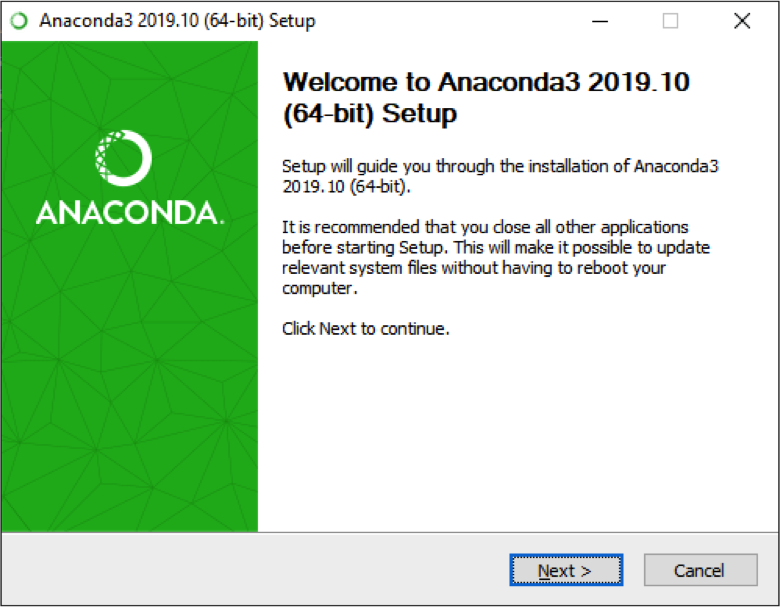
\includegraphics[width=0.67\textwidth]{python003.png}
\end{figure}
\end{itemize}
\begin{tikzpicture}[remember picture, overlay]
\draw[draw=red,rounded corners=2pt,line width=1pt]  (6.9,0.7) rectangle ++(1.3,0.5);
\end{tikzpicture}
\end{frame}

\begin{frame}{How to install Anaconda?}
\begin{itemize}
\item Click on {\color{red}I Agree}.
\begin{figure}
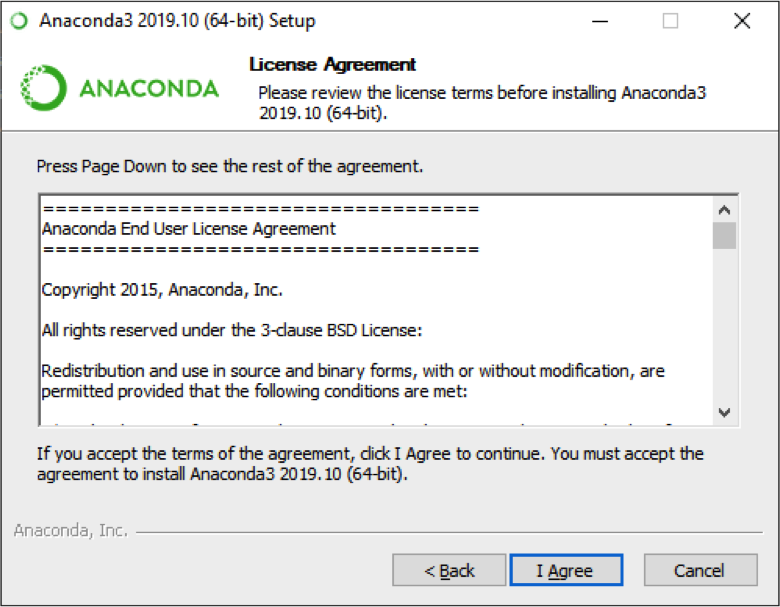
\includegraphics[width=0.7\textwidth]{python004.png}
\end{figure}
\end{itemize}
\begin{tikzpicture}[remember picture, overlay]
\draw[draw=red,rounded corners=2pt,line width=1pt]  (6.9,0.7) rectangle ++(1.3,0.5);
\end{tikzpicture}
\end{frame}

\begin{frame}{How to install Anaconda?}
\begin{itemize}
\item Click on {\color{red}Next}.
\begin{figure}
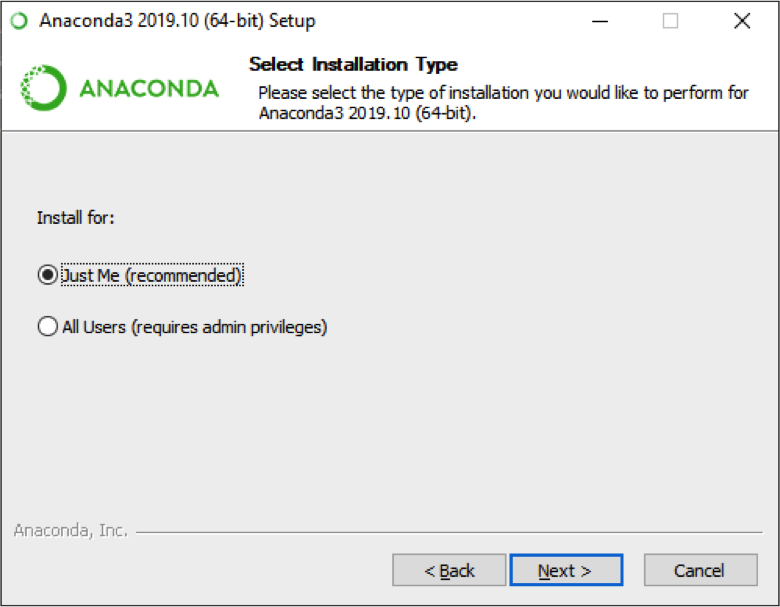
\includegraphics[width=0.7\textwidth]{python005.png}
\end{figure}
\end{itemize}
\begin{tikzpicture}[remember picture, overlay]
\draw[draw=red,rounded corners=2pt,line width=1pt]  (6.9,0.7) rectangle ++(1.3,0.5);
\end{tikzpicture}
\end{frame}

\begin{frame}{How to install Anaconda?}
\begin{itemize}
\item Click on {\color{red}Install}.

\begin{figure}
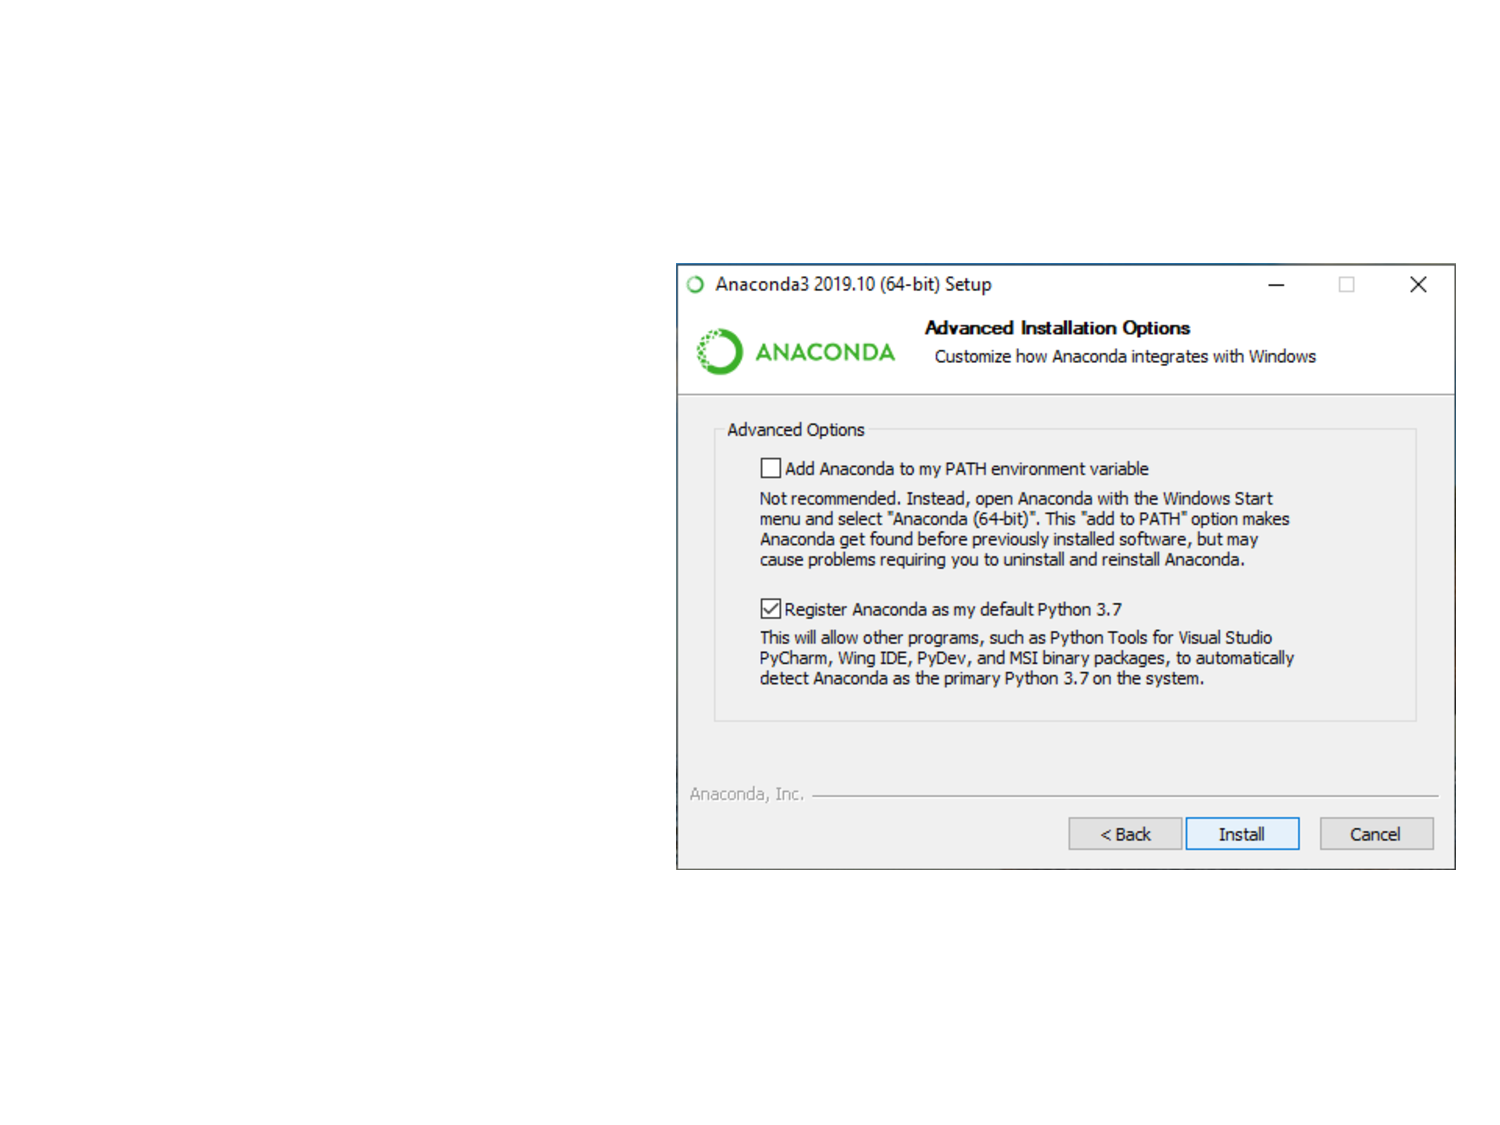
\includegraphics[width=0.7\textwidth]{AnacondaInstallation}
\end{figure}
\end{itemize}
\begin{tikzpicture}[remember picture, overlay]
\draw[draw=red,rounded corners=2pt,line width=1pt]  (6.9,0.7) rectangle ++(1.3,0.5);
\end{tikzpicture}
\end{frame}

\begin{frame}{How to install Anaconda?}
\begin{itemize}
\item Click on {\color{red}Next}.
\begin{figure}
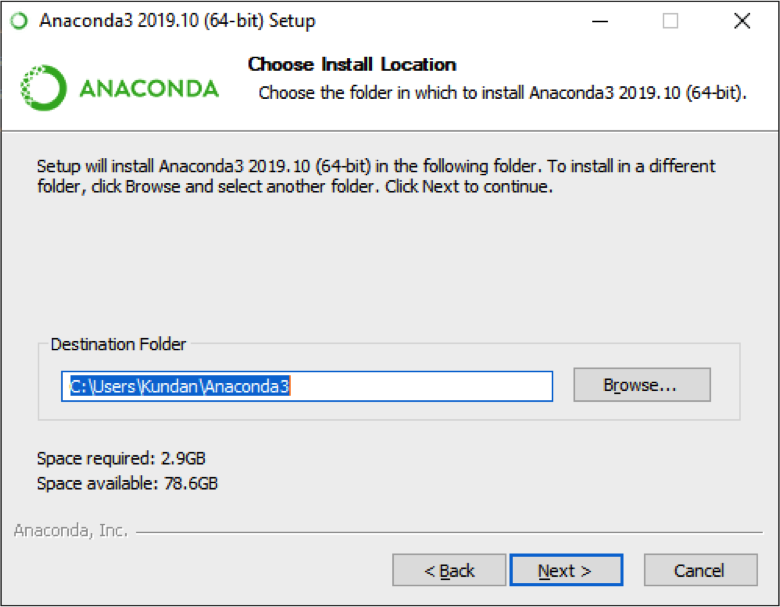
\includegraphics[width=0.7\textwidth]{python006.png}
\end{figure}
\end{itemize}
\begin{tikzpicture}[remember picture, overlay]
\draw[draw=red,rounded corners=2pt,line width=1pt]  (6.9,0.7) rectangle ++(1.3,0.5);
\end{tikzpicture}
\end{frame}

\begin{frame}{How to install Anaconda?}
\begin{itemize}
\item Click on {\color{red}Next}, when it gets highlighted.
\begin{figure}
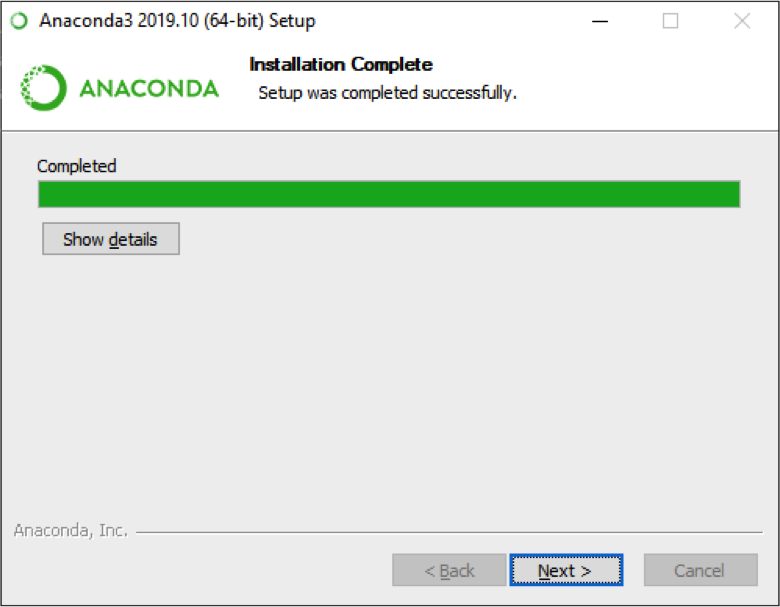
\includegraphics[width=0.7\textwidth]{python007.png}
\end{figure}
\end{itemize}
\begin{tikzpicture}[remember picture, overlay]
\draw[draw=red,rounded corners=2pt,line width=1pt]  (6.9,0.7) rectangle ++(1.3,0.5);
\end{tikzpicture}
\end{frame}

\begin{frame}{How to install Anaconda?}
\begin{itemize}
\item Click on {\color{red}Next}.
\begin{figure}
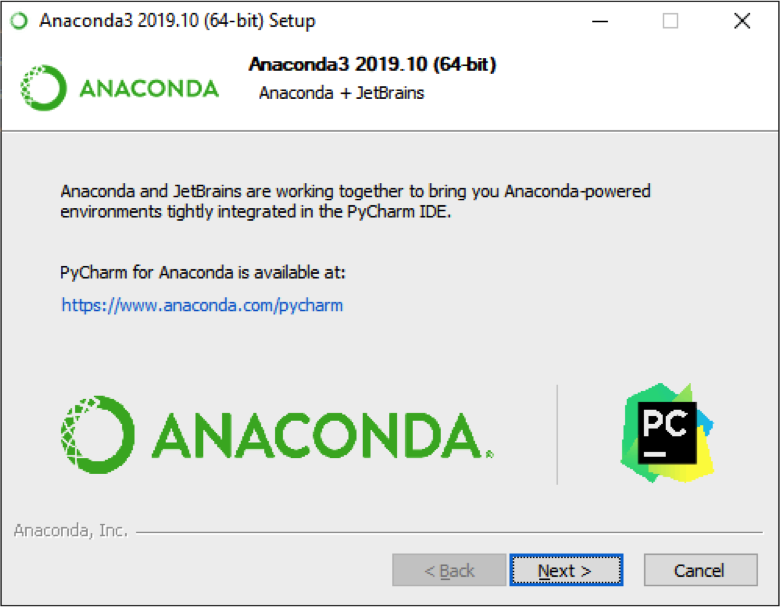
\includegraphics[width=0.7\textwidth]{python008.png}
\end{figure}
\end{itemize}
\begin{tikzpicture}[remember picture, overlay]
\draw[draw=red,rounded corners=2pt,line width=1pt]  (6.9,0.7) rectangle ++(1.3,0.5);
\end{tikzpicture}
\end{frame}

\begin{frame}{How to install Anaconda?}
\begin{itemize}
\item Click on {\color{red}Finish}.
\begin{figure}
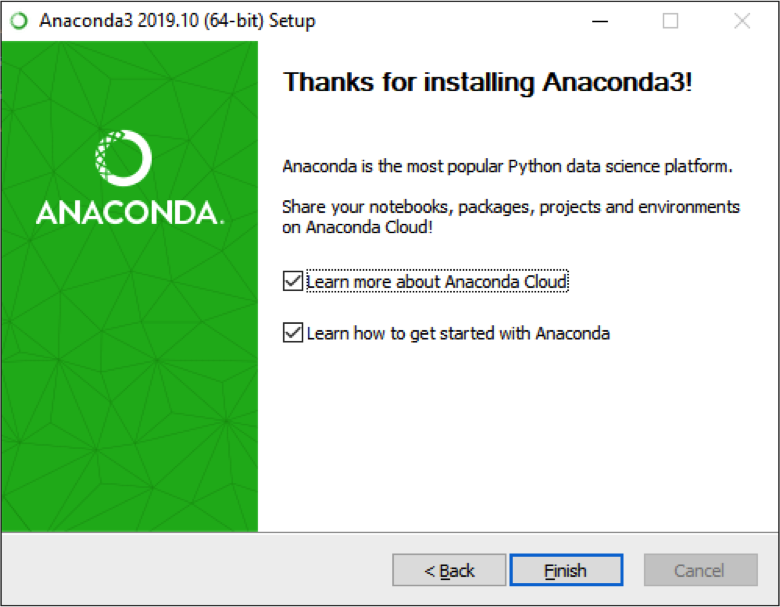
\includegraphics[width=0.7\textwidth]{python009.png}
\end{figure}
\end{itemize}
\begin{tikzpicture}[remember picture, overlay]
\draw[draw=red,rounded corners=2pt,line width=1pt]  (6.9,0.7) rectangle ++(1.3,0.5);
\end{tikzpicture}
\end{frame}

\section{Open Jupyter-Notebook}
\subsection{}

\begin{frame}{Open Anaconda Powershell Prompt}
\begin{itemize}
\item Go to start (bottom-left corner) and scroll down to find {\color{red}Anaconda3 (64 bit)}.
\item Click on {\color{red}Anaconda Powershell Promt} to open it.
\begin{figure}
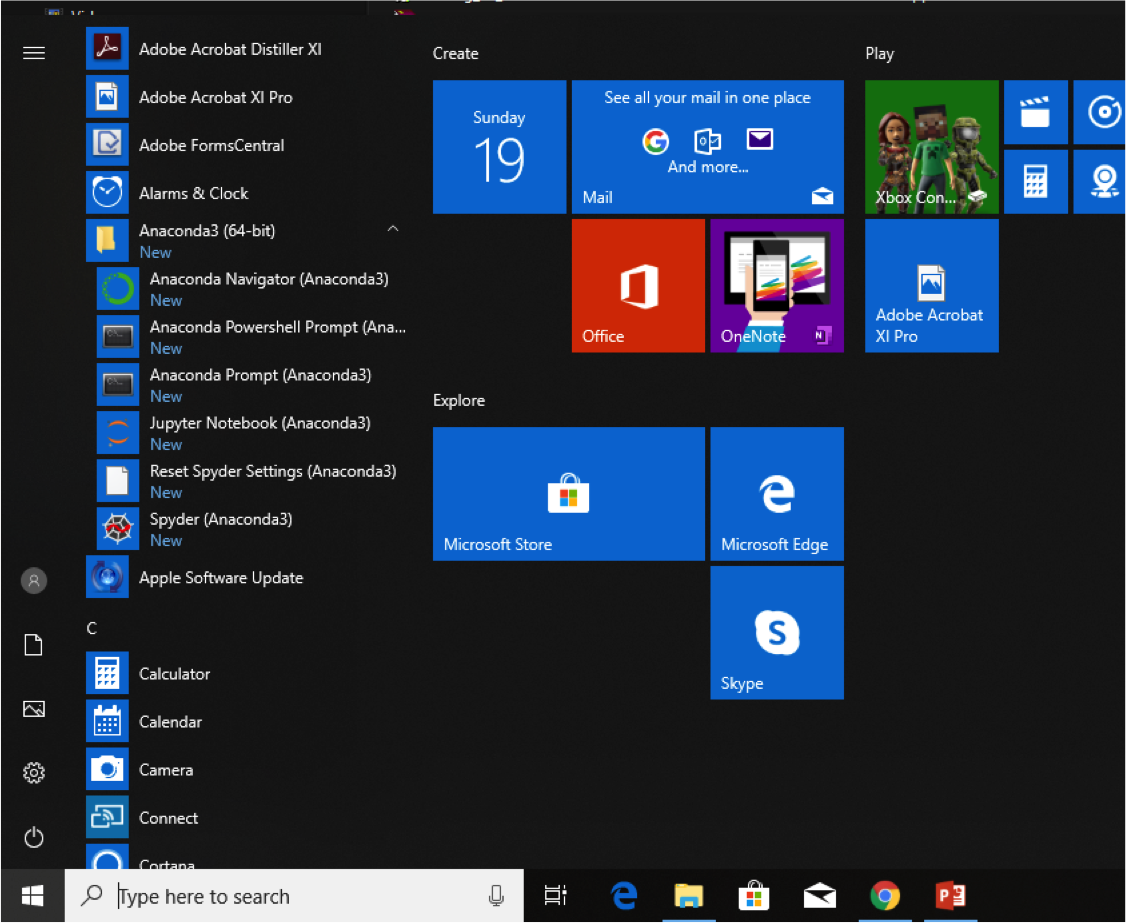
\includegraphics[width=0.63\textwidth]{python010.png}
\end{figure}
\end{itemize}
\end{frame}

%
%%\lstset{language=Python}
%%\lstset{frame=lines}
%%\lstset{caption={Insert code directly in your document}}
%%\lstset{label={lst:code_direct}}
%%\lstset{basicstyle=\footnotesize}
%

\begin{frame}{Check, is anaconda in path?}
\begin{itemize}
\item In the powershell prompt {\color{red}run ``conda''} to ensure that anaconda is in path.

\begin{center}
{\color{blue}\$ conda}
\end{center}
\begin{figure}
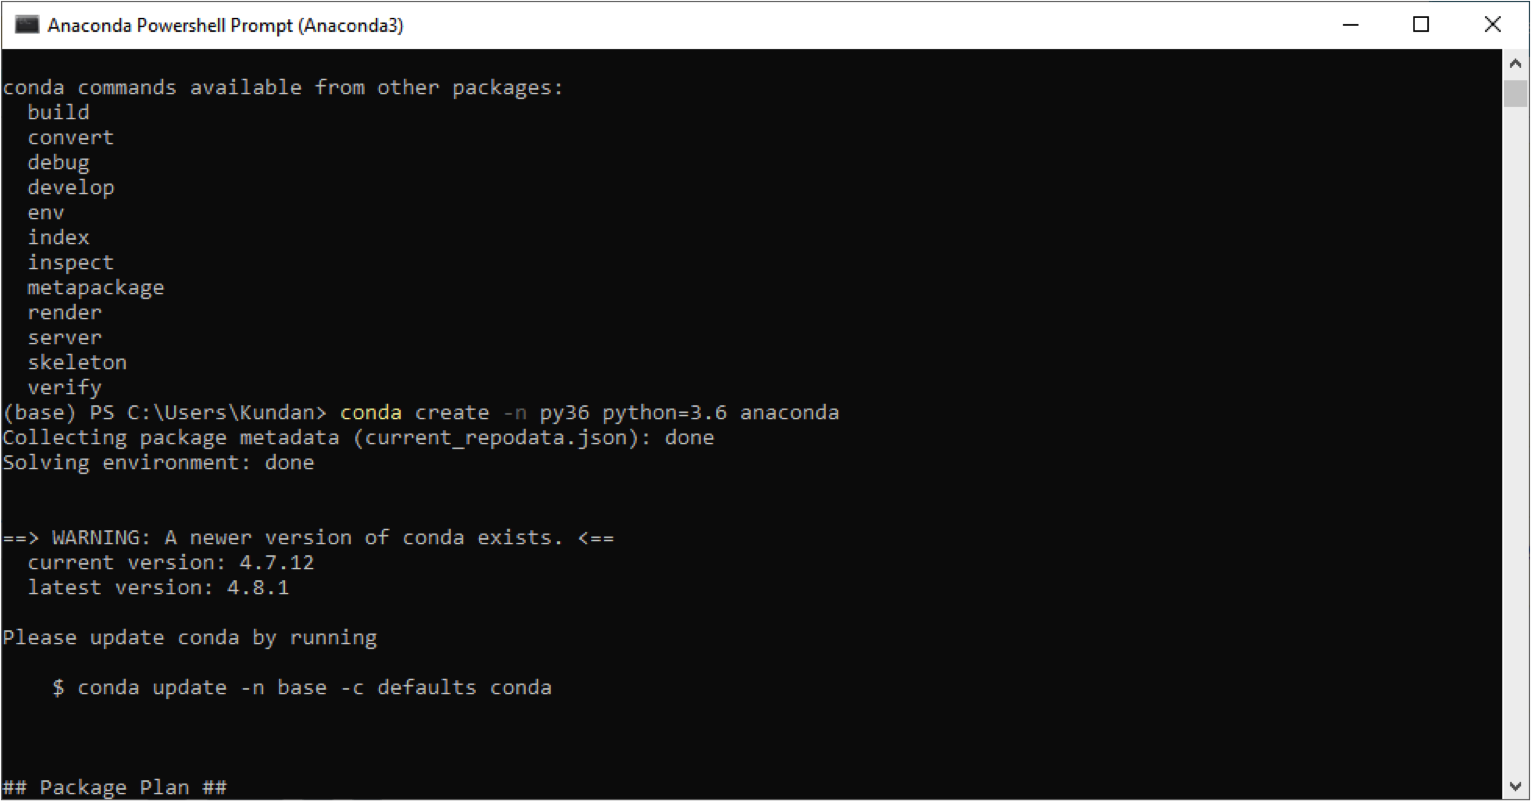
\includegraphics[width=0.9\textwidth]{python011.png}
\end{figure}
\end{itemize}
\end{frame}

\begin{frame}{How to create a virtual environment?}
\begin{itemize}
\item To create a virtual environment run

\begin{center}
{\color{blue}\$ conda create -n py36 python=3.6 anaconda}
\end{center}

\item press {\color{red}Y} to proceed. Wait for complete the installation.

\item After the completion of the installation, activate the virtual environment as
 
\begin{center}
{\color{blue}\$ conda activate py36}
\end{center} 
      
\item Ensure that default environment base is changed to py36.

\item To deactivate the environment

\begin{center}
{\color{blue}\$ conda deactivate}
\end{center} 
\end{itemize}
\textbf{\color{red}NOTE: }  You can use up and down key in the keyboard to see command history executed.
\end{frame}

\begin{frame}{How to switch to other environment?}
\begin{itemize}
\item Start Jupyter-Notebook by running command.

 \item A localhost will open in default browser with address

%\begin{center}
%http://localhost:8888/tree  (number may vary system to system)
%\end{center}

\item Browser will show your directories. You can create your project directory and can start coding by creating New notebook (right-top side of the screen)

\end{itemize}
\end{frame}

{
\setbeamertemplate{logo}{}
\makeatletter
\setbeamertemplate{footline}{
        \leavevmode%
  
  % First line.
  \hbox{%
  \begin{beamercolorbox}[wd=.2\paperwidth,ht=\beamer@decolines@lineup,dp=0pt]{}%
  \end{beamercolorbox}%
  \begin{beamercolorbox}[wd=.8\paperwidth,ht=\beamer@decolines@lineup,dp=0pt]{lineup}%
  \end{beamercolorbox}%
  } %
  % Second line.
  \hbox{%
  \begin{beamercolorbox}[wd=\paperwidth,ht=\beamer@decolines@linemid,dp=0pt]{linemid}%
  \end{beamercolorbox}%
  } %
  % Third line.
  \hbox{%
  \begin{beamercolorbox}[wd=.1\paperwidth,ht=\beamer@decolines@linebottom,dp=0pt]{}%
  \end{beamercolorbox}%
  \begin{beamercolorbox}[wd=.9\paperwidth,ht=\beamer@decolines@linebottom,dp=0pt]{linebottom}%
  \end{beamercolorbox}%
  }%
        }
\makeatother

\begin{frame}
\centering
\includegraphics[width=0.4\paperwidth]{queries.jpg}\\
\includegraphics[width=0.5\paperwidth]{thank_you.png}
\end{frame}
}




